\documentclass[12pt,a4paper]{article}

% Packages
\usepackage{
    amsmath,
    amssymb,
    graphicx,
    titletoc,
    fancyhdr,
    geometry,
    babel,
    xcolor,
    enumerate,
    fix-cm,
    tocbibind,
    listings,
    float,
    enumitem,
    subcaption,
    hyperref
}

% Define colors
\definecolor{vgreen}{RGB}{104,180,104}
\definecolor{vblue}{RGB}{49,49,255}
\definecolor{vorange}{RGB}{255,143,102}

% Listings customization
\renewcommand\lstlistingname{Figura}
\renewcommand\lstlistlistingname{Figura}

\makeatletter
\newcommand*\@lbracket{[}
\newcommand*\@rbracket{]}
\newcommand*\@colon{:}
\newcommand*\colorIndex{%
    \edef\@temp{\the\lst@token}%
    \ifx\@temp\@lbracket \color{black}%
    \else\ifx\@temp\@rbracket \color{black}%
    \else\ifx\@temp\@colon \color{black}%
    \else \color{vorange}%
    \fi\fi\fi
}
\makeatother

% Setup for listings
\lstset{
    captionpos=b,
    belowcaptionskip=\bigskipamount,
    frame=single,
    basicstyle=\small\ttfamily,
    numbers=left,
    numberstyle=\tiny\color{gray},
    xleftmargin=2em,
    framexleftmargin=2em,
    backgroundcolor=\color{vgreen!10},
    stepnumber=1,
    showstringspaces=false,
    keywordstyle=\color{vblue},
    commentstyle=\color{gray},
    stringstyle=\color{vorange},
}

\begin{document}

\begin{titlepage}
    \centering
    
\includegraphics[scale=1]{M2_Modelos_de_Programación/reporte/figuras/Logo_Tec.png}\\
    \vspace{.5cm}
    \bfseries\large Escuela de Ingeniería y Ciencias
        
    \vspace{5cm}
    \centering
    \textbf{\Huge Cómputo en la Nube}
    \vspace{0.5cm}
        
    {\Large Programación de una Solución Paralela}

    \vspace{5cm}
        
    \textbf{\LARGE Armando Bringas Corpus}
        
    \vspace{0.5cm}
        
    {\large A01200230}
        
    \vfill
        
\end{titlepage}

\section{Introducción}


\section{Liga al repositorio}

\begin{itemize}
    \item Repositorio General: \url{https://github.com/armandoBringas/Cloud_Computing}
    \item Código original de la actividad: \url{https://github.com/armandoBringas/Cloud_Computing/tree/main/M2_Modelos_de_Programaci%C3%B3n/PruebaOMP_original}
    \item Código refactorizado de la actividad: \url{https://github.com/armandoBringas/Cloud_Computing/tree/main/M2_Modelos_de_Programaci%C3%B3n/PruebaOMP_refactorizado}
\end{itemize}


\section{Capturas de pantalla}
Con el código original de la actividad utilizando los siguientes parámetros se obtuvieron los siguientes resultados:

\vspace{1em}

\textbf{Ejemplo 1 - Código original:}

\begin{lstlisting}[language=C, numbers=none]
#define N 1000
#define chunk 150
#define mostrar 20
\end{lstlisting}

\begin{figure}[H]
    \centering
    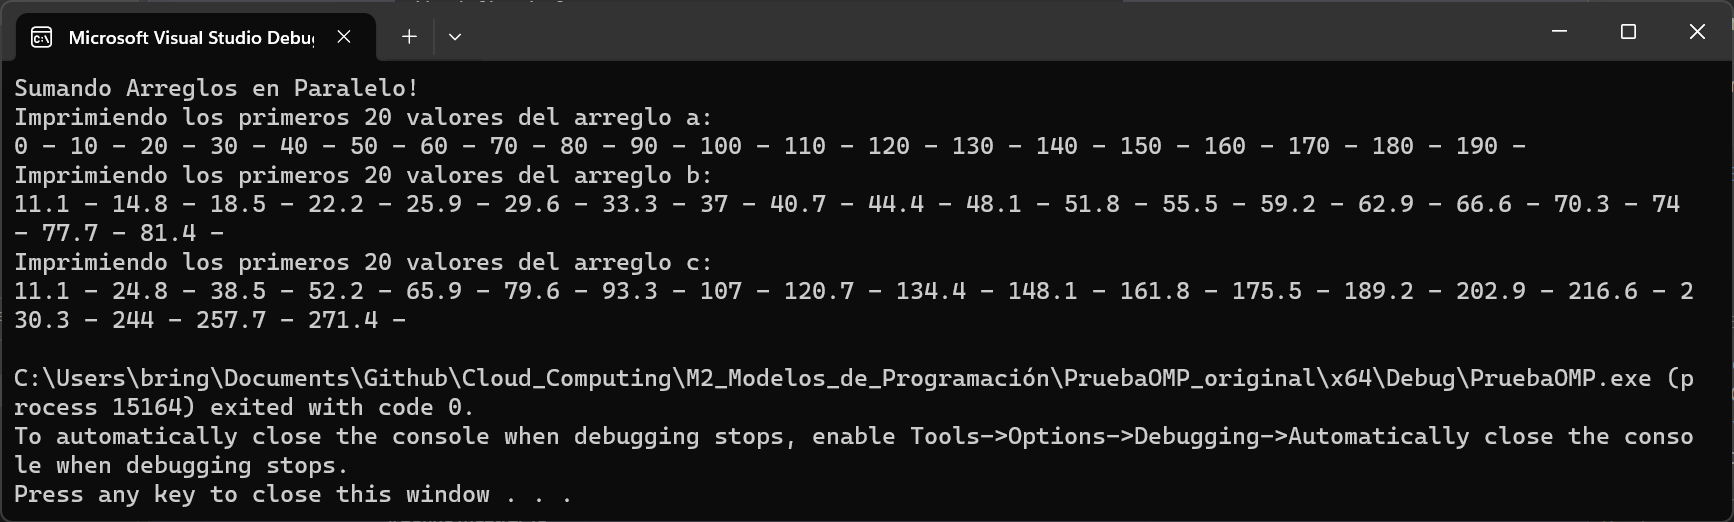
\includegraphics[width=1\linewidth]{M2_Modelos_de_Programación/reporte/figuras/Código_original_ejemplo-1.png}
    \captionof{lstlisting}{Salida del Ejemplo 1 - Código original}
    \label{fig:Código_original_ejemplo-1}
\end{figure}

\textbf{Ejemplo 2 - Código original:}

\begin{lstlisting}[language=C, numbers=none]
#define N 20000
#define chunk 500
#define mostrar 75
\end{lstlisting}

\begin{figure}[H]
    \centering
    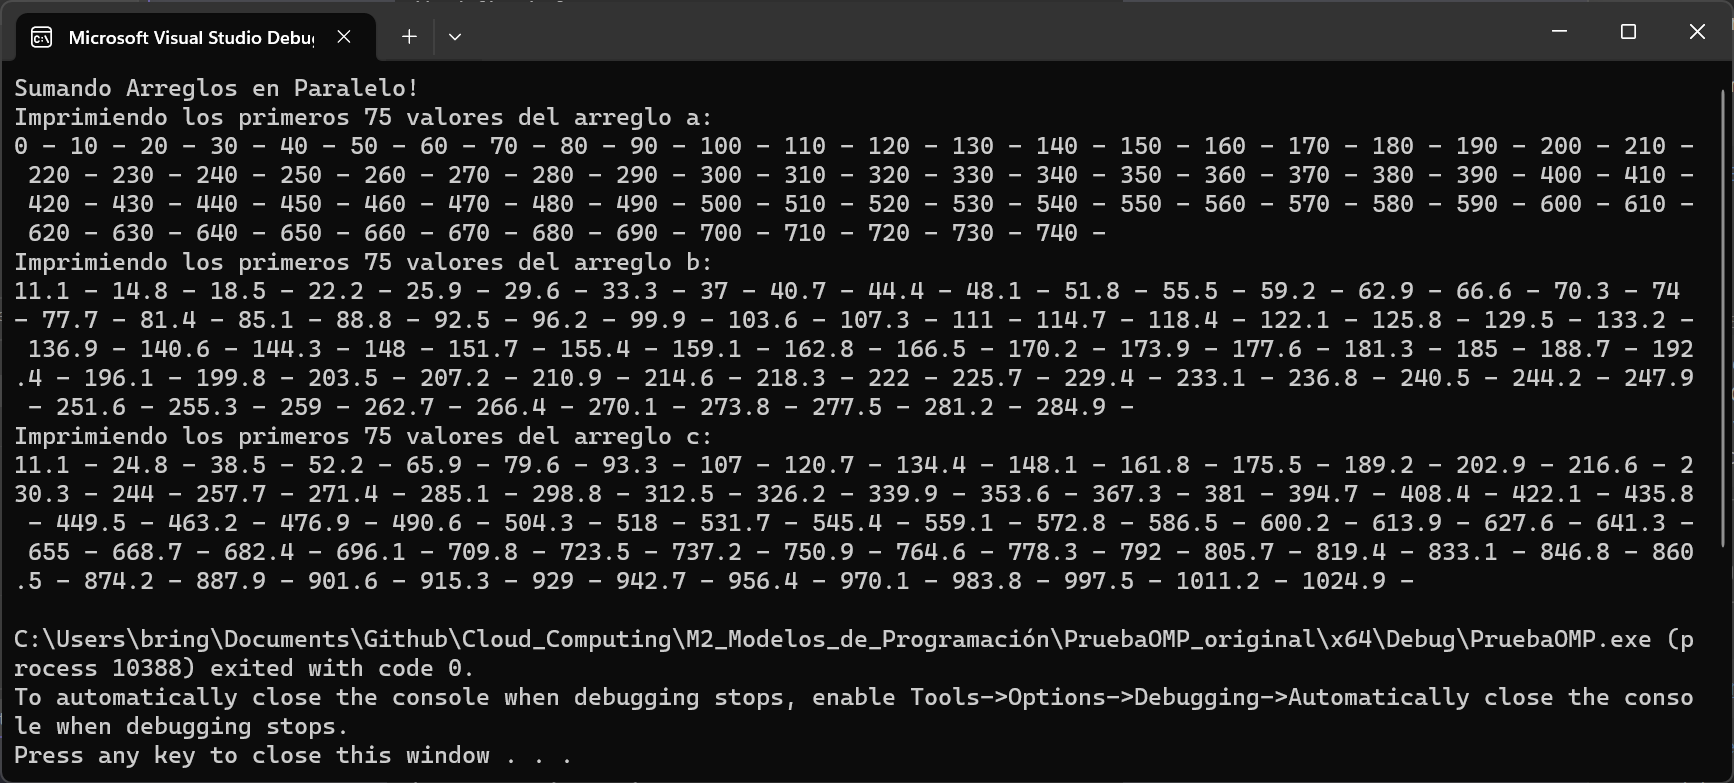
\includegraphics[width=1\linewidth]{M2_Modelos_de_Programación/reporte/figuras/Código_original_ejemplo-2.png}
    \captionof{lstlisting}{Salida del Ejemplo 2 - Código original}
    \label{fig:Código_original_ejemplo-2}
\end{figure}

Se realizaron algunas refactorizaciones del código original de la actividad que en la siguiente sección serán explicadas. En este código refactorizado se implementó la opción mediante una macro de ejecución el poder correr los valores de los parámetros definidos dentro del código o que estos se seleccionaran de forma aleatoria dentro de un rango definido.

\vspace{1em}

Rangos seleccionados para los ejemplos usando el código refactorizado:

\begin{lstlisting}[language=C, numbers=none]
const int N = numeroAleatorio(50000, 60000);
const int CHUNK_SIZE = numeroAleatorio(700, 1000);
const int MOSTRAR = numeroAleatorio(10, 25);
\end{lstlisting}

\vspace{1em}

Con el código refactorizado de la actividad se obtuvieron los siguientes resultados:

\vspace{1em}

\textbf{Ejemplo 1 - Código refactorizado:}

\begin{figure}[H]
    \centering
    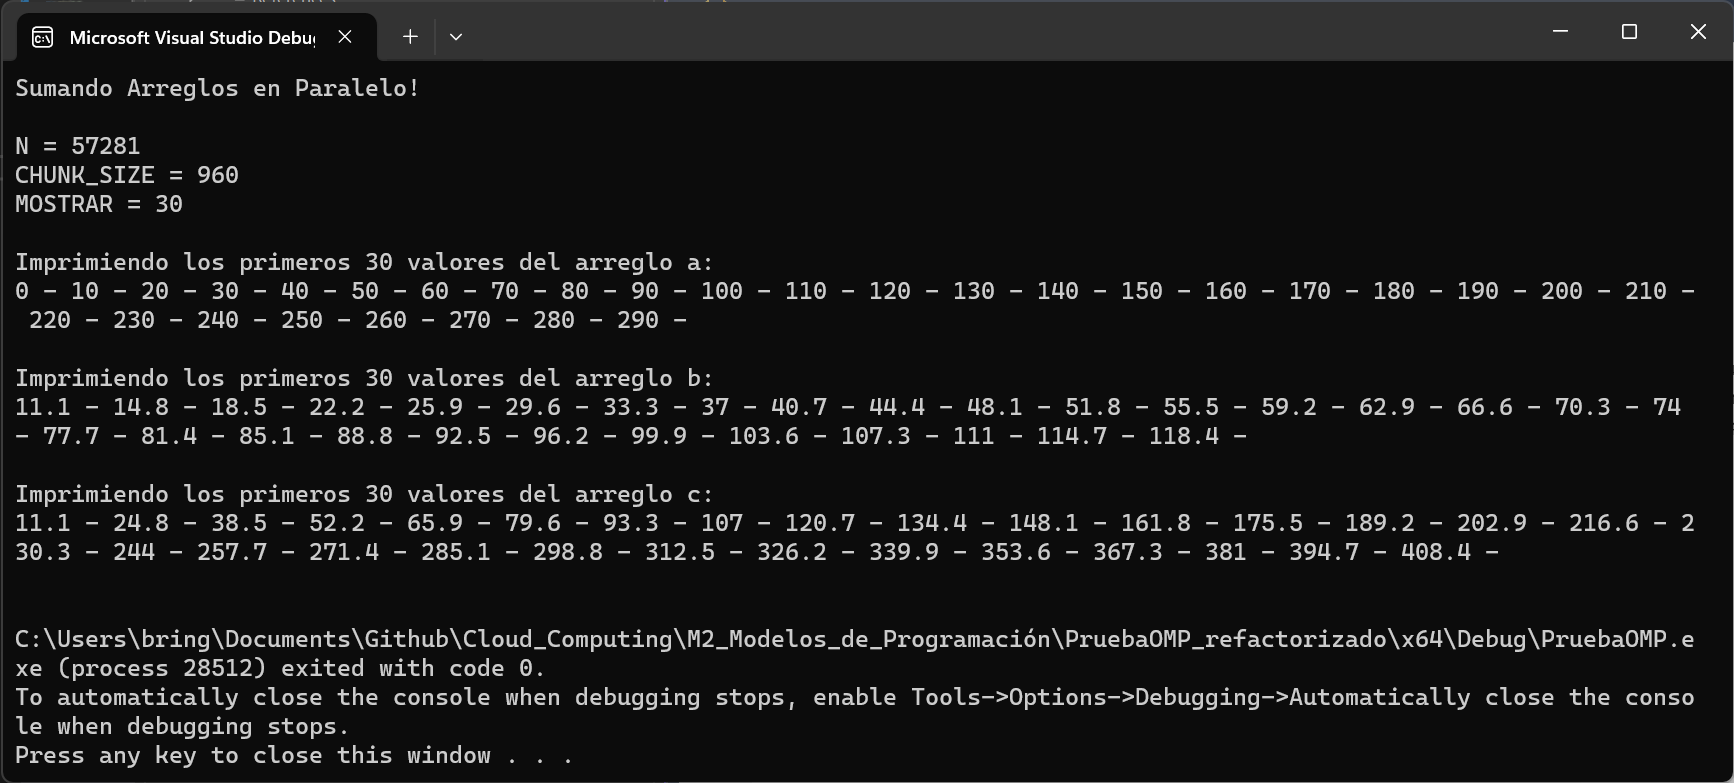
\includegraphics[width=1\linewidth]{M2_Modelos_de_Programación/reporte/figuras/Código_refactorizado_ejemplo-1.png}
    \captionof{lstlisting}{Salida del Ejemplo 1 - Código refactorizado}
    \label{fig:Código_refactorizado_ejemplo-1}
\end{figure}


\textbf{Ejemplo 2 - Código refactorizado:}

\begin{figure}[H]
    \centering
    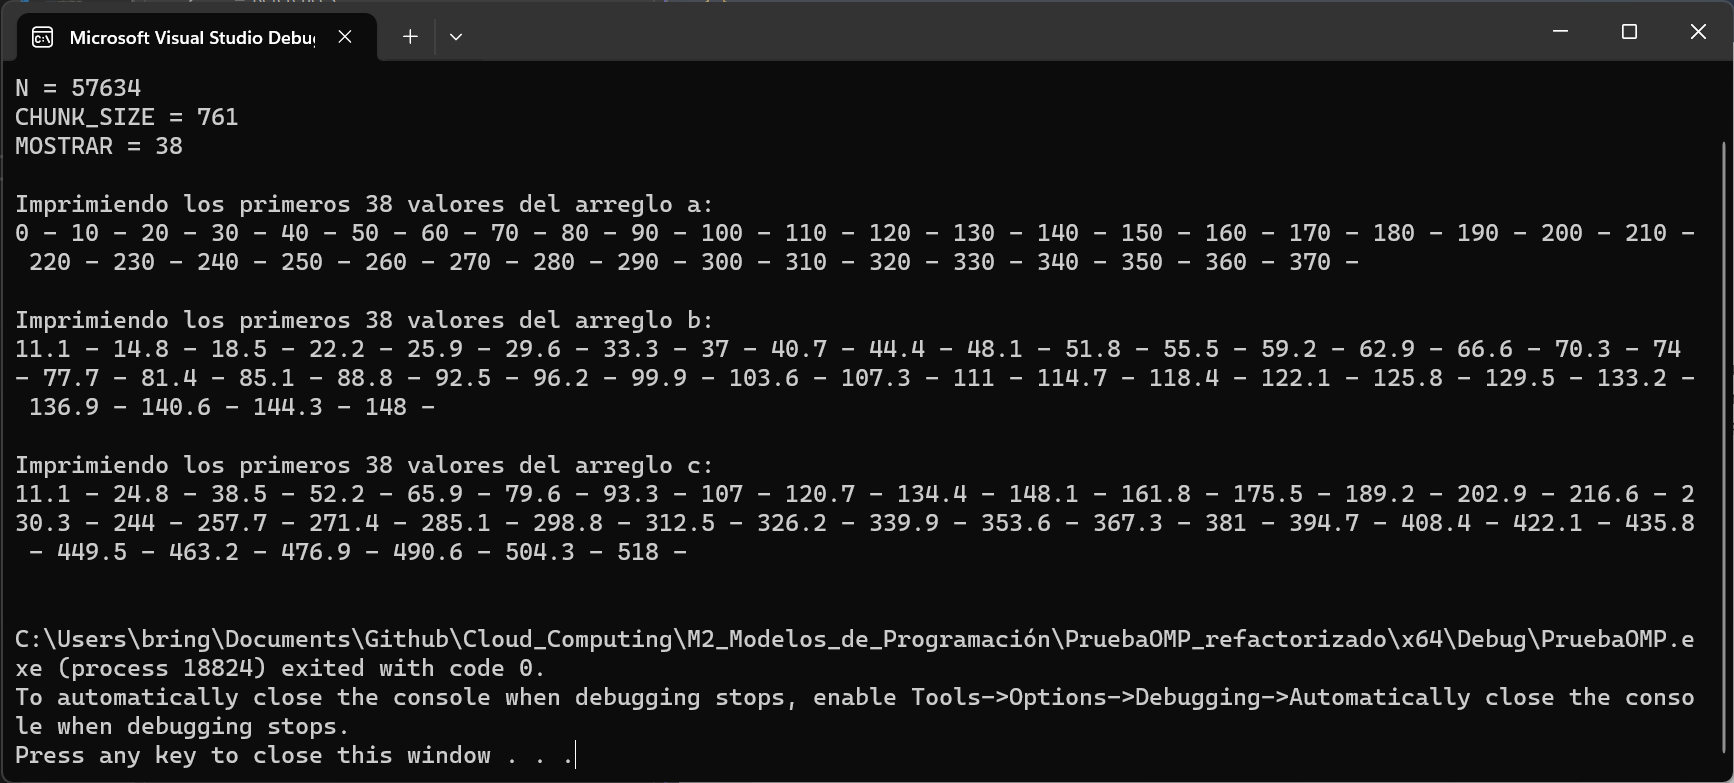
\includegraphics[width=1\linewidth]{M2_Modelos_de_Programación/reporte/figuras/Código_refactorizado_ejemplo-2.png}
    \captionof{lstlisting}{Salida del Ejemplo 2 - Código refactorizado}
    \label{fig:Código_refactorizado_ejemplo-2}
\end{figure}


\section{Explicación del código y resultados}

\textbf{Código original}

\vspace{1em}

Por medio del código que se implementó en la práctica se buscó ejemplificar el uso del \textbf{paralelismo a nivel de instrucción} en la cual a través de la librería OpenMP buscamos ejecutar más de una instrucción a la vez, es decir, en paralelo.

\vspace{1em}

Al inicio del código se definen tres directivas del preprocesador (macros) las cuales serán empleadas para modificar la distribución de la carga entre los hilos del procesador:

\begin{lstlisting}[language=C, numbers=none]
#define N 20000
#define chunk 500
#define mostrar 75
\end{lstlisting}
En donde,
\begin{itemize}
    \item \texttt{N}: Es la cantidad de elementos que se manejaran en los arreglos.
    \item \texttt{chunk}: El tamaño de los pedazos de los arreglos para que cada hilo creado maneje esta cantidad específica de elementos.
    \item \texttt{mostrar}: Es la cantidad los elementos a imprimir de la operación que se hará con los arreglos
\end{itemize}

Posteriormente se define el prototipo de la función que imprimirá los arreglos que se definan en el programa, esta función recibe un puntero el cual hace referencia al arreglo que se le da de entrada.

\begin{lstlisting}[language=C, numbers=none]
void imprimeArreglo(float* d);
\end{lstlisting}

\vspace{1em}

En nuestra función \texttt{main()} la cual es la rutina principal del programa se hace la definición de los arreglos en los cuales los arreglos \texttt{a} y \texttt{b} se les asignarán los valores a cada uno de sus elementos por medio de un bucle y una operación establecida para facilitar la populación de los arreglos, el arreglo \texttt{c} es el que contendrá el resultado de la suma de los arreglos \texttt{a} y \texttt{b}. El tamaño de cada uno de los arreglos estará establecido por constante \texttt{N}.

\begin{lstlisting}[language=C, numbers=none]
int main()
{
    std::cout << "Sumando Arreglos en Paralelo!\n";
    float a[N], b[N], c[N];
    int i;

    for (int i = 0; i < N; i++)
    {
        a[i] = i * 10;
        b[i] = (i + 3) * 3.7;
    }
\end{lstlisting}

\vspace{1em}

En la siguiente porción de código se inicia el proceso de paralelización a través de la librería \textbf{OpenMP}, con la cual el bucle \texttt{for} sera el que se esté paralelizando. De igual manera, se establece la información que se compartirá entre las diversas particiones a través de la función \texttt{shared} la cual recibirá como parámetros los arreglos y la variable \texttt{pedazos} a la cual se le asigna como valor la constante \texttt{chunk}, esta variable se encargará de guardar el valor de cómo será repartida la información a través de los hilos que sean creados. Es importante resaltar que la variable \texttt{i} se debe mantener privada para que los ciclos no se puedan mezclar con otros hilos. De igual manera establecemos el \texttt{schedule} como estático para que siempre sea ejecutado de la misma manera.

\begin{lstlisting}[language=C, numbers=none]
    int pedazos = chunk;

    #pragma omp parallel for \
    shared(a, b, c, pedazos) private(i) \
    schedule(static, pedazos)
    for (int i = 0; i < N; i++)
        c[i] = a[i] + b[i];
\end{lstlisting}

\vspace{1em}

A continuación hacemos uso de la función \texttt{imprimeArreglo()} para imprimir los arreglos con el número de elementos que se definió en la constante \texttt{mostrar}.

\begin{lstlisting}[language=C, numbers=none]
    std::cout << "Imprimiendo los primeros " << mostrar 
              << " valores del arreglo a: " << std::endl;
    imprimeArreglo(a);

    std::cout << "Imprimiendo los primeros " << mostrar 
              << " valores del arreglo b: " << std::endl;
    imprimeArreglo(b);

    std::cout << "Imprimiendo los primeros " << mostrar 
              << " valores del arreglo c: " << std::endl;
    imprimeArreglo(c);

    return 0;
}
\end{lstlisting}

\vspace{1em}

Finalmente se tiene la función que imprime cada uno de los elementos del arreglo que recibe como puntero.

\begin{lstlisting}[language=C, numbers=none]
void imprimeArreglo(float* d)
{
    for (int x = 0; x < mostrar; x++)
        std::cout << d[x] << " - ";
    std::cout << std::endl;
}
\end{lstlisting}

\vspace{1em}

\textbf{Código refactorizado}

\vspace{1em}

Como se comentó en la sección anterior se realizó un código en el cual se efectuaron algunas refactorizaciones para tener a través de una macro de ejecución el poder ejecutar los valores de los parámetros \texttt{N, chunk, mostrar}  de forma aleatoria dentro de un rango definido o de una forma establecida. De igual manera se separaron los prototipos para ser definidos en un archivo de cabecera y se buscó modularizar el código para en futuro de ser reutilizado poder más fácil poder depurarlo al tener funciones separadas.

Otro cambio importante es que tuvimos que cambiar la definición de los arreglos como vectores para poder tener arreglos dinámicos y evitar errores en la compilación y ejecución del código.

\vspace{1em}
 
\begin{lstlisting}[language=C, numbers=none]
#ifndef PRUEBA_OMP_H
#define PRUEBA_OMP_H

void imprimeArreglo(const std::vector<float>& d);
void sumaArreglosParalelo(const std::vector<float>& a, 
                          const std::vector<float>& b, 
                          std::vector<float>& c, 
                          int size,
                          int chunk);
int numeroAleatorio(int min_num, int max_num);

#endif
\end{lstlisting}



\begin{lstlisting}[language=C, numbers=none]
#include <iostream>
#include <omp.h>
#include <stdio.h>
#include <vector>
#include "PruebaOMP.h"

// Comentar para usar valores predefinidos
#define USE_RANDOM_VALUES 

#ifdef USE_RANDOM_VALUES
const int N = numeroAleatorio(50000, 60000);
const int CHUNK_SIZE = numeroAleatorio(700, 1000);
const int MOSTRAR = numeroAleatorio(20, 40);
#else
const int N = 1000;
const int CHUNK_SIZE = 100;
const int MOSTRAR = 10;
#endif

int main()
{
    std::cout << "Sumando Arreglos en Paralelo!\n";
    std::cout << std::endl;
    std::cout << "N = " << N << std::endl;
    std::cout << "CHUNK_SIZE = " << CHUNK_SIZE 
              << std::endl;
    std::cout << "MOSTRAR = " << MOSTRAR 
              << std::endl;
    std::cout << std::endl;

    std::vector<float> a(N), b(N), c(N);

    for (int i = 0; i < N; i++)
    {
        a[i] = i * 10;
        b[i] = (i + 3) * 3.7;
    }

    sumaArreglosParalelo(a, b, c, N, CHUNK_SIZE);

    std::cout << "Imprimiendo los primeros " << MOSTRAR 
              << " valores del arreglo a: " << std::endl;
    imprimeArreglo(a);

    std::cout << "Imprimiendo los primeros " << MOSTRAR 
              << " valores del arreglo b: " << std::endl;
    imprimeArreglo(b);

    std::cout << "Imprimiendo los primeros " << MOSTRAR 
              << " valores del arreglo c: " << std::endl;
    imprimeArreglo(c);

    return 0;
}

void imprimeArreglo(const std::vector<float>& d)
{
    for (int x = 0; x < MOSTRAR && x < d.size(); x++)
        std::cout << d[x] << " - ";

    std::cout << std::endl;
    std::cout << std::endl;
}

void sumaArreglosParalelo(const std::vector<float>& a, 
                          const std::vector<float>& b,
                          std::vector<float>& c, int n, 
                          int chunk)
{
#pragma omp parallel for \
    shared(a, b, c, chunk) \
    schedule(static, chunk)
    for (int i = 0; i < n; i++)
        c[i] = a[i] + b[i];
}

int numeroAleatorio(int min_num, int max_num)
{
    // Ensure a valid range
    if (min_num >= max_num) {
        std::swap(min_num, max_num);
    }

    static bool seed_initialized = false;
    if (!seed_initialized) {
        srand(static_cast<unsigned>(time(nullptr)));
        seed_initialized = true;
    }

    return rand() % (max_num - min_num + 1) + min_num;
}
\end{lstlisting}

\vspace{1em}

\textbf{Resultados}

\vspace{1em}

Para experimentar tanto con el código original como con el que se refactorizó, vamos a modificar en ambos las ecuaciones para popular los arreglos \texttt{a} y \texttt{b}, en este caso quedan definidos como:

\begin{lstlisting}[language=C, numbers=none]
    for (int i = 0; i < N; i++)
    {
        a[i] = (i + 25) * 48.6; // (i + 2) * 10;
        b[i] = (i + 77) * 150.7; // (i + 3) * 3.7;
    }
\end{lstlisting}

Y establecemos de igual manera en ambos códigos las constantes \texttt{N, chunk, mostrar} con los siguientes valores:

\begin{lstlisting}[language=C, numbers=none]
#define N 1000
#define chunk 500
#define mostrar 50
\end{lstlisting}

\vspace{1em}

Para el código original obtenemos los siguientes resultados:

\begin{figure}[H]
    \centering
    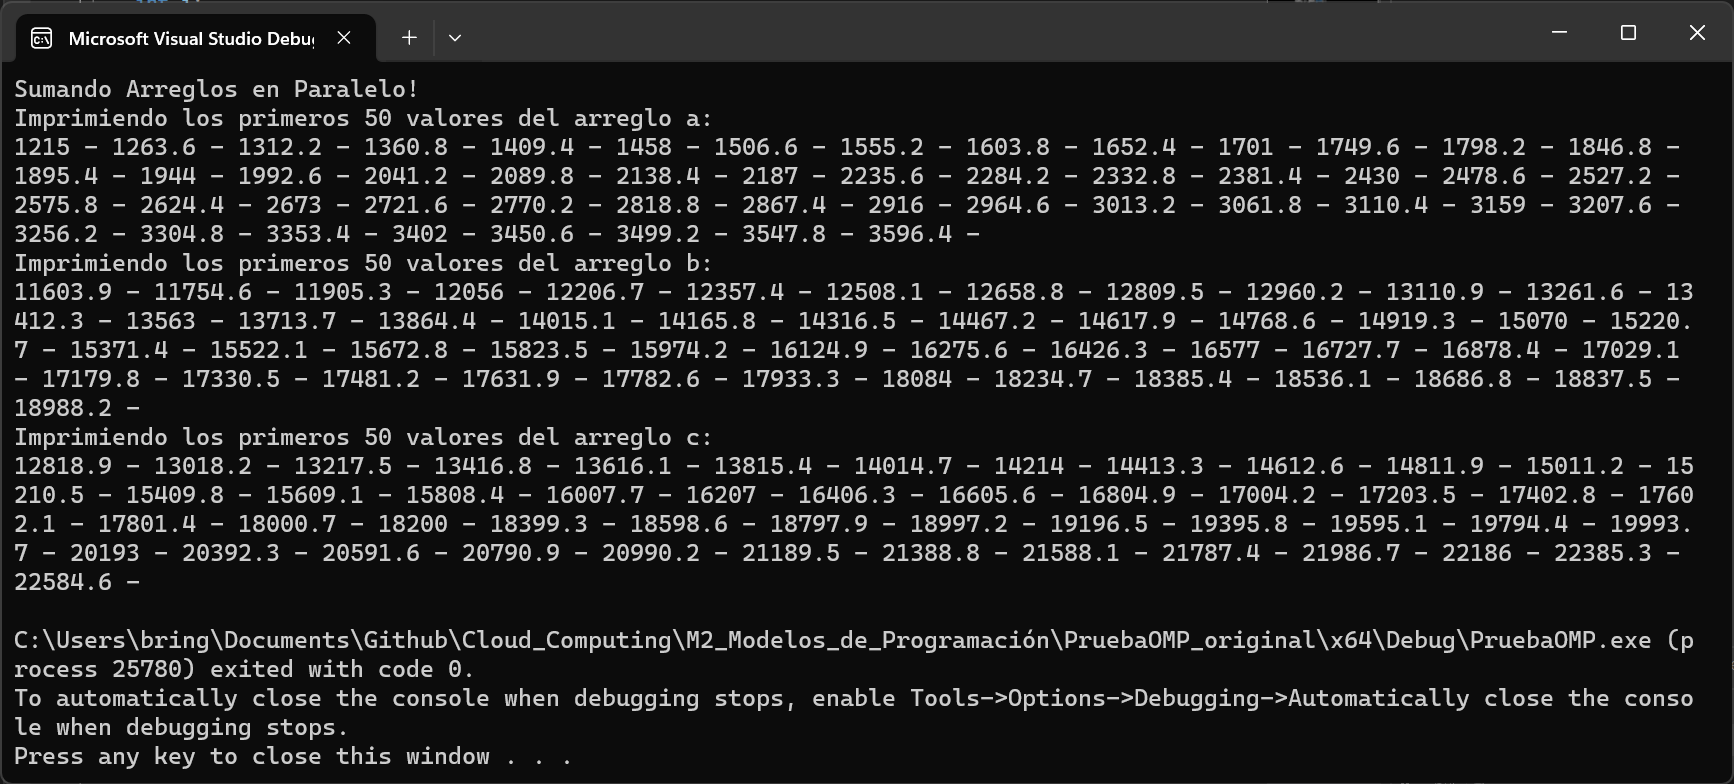
\includegraphics[width=1\linewidth]{M2_Modelos_de_Programación/reporte/figuras/Código_original_resultados.png}
    \captionof{lstlisting}{Resultados del Código original}
    \label{fig:Código_original_resultados}
\end{figure}

Para el código refactorizado obtenemos los siguientes resultados:

\begin{figure}[H]
    \centering
    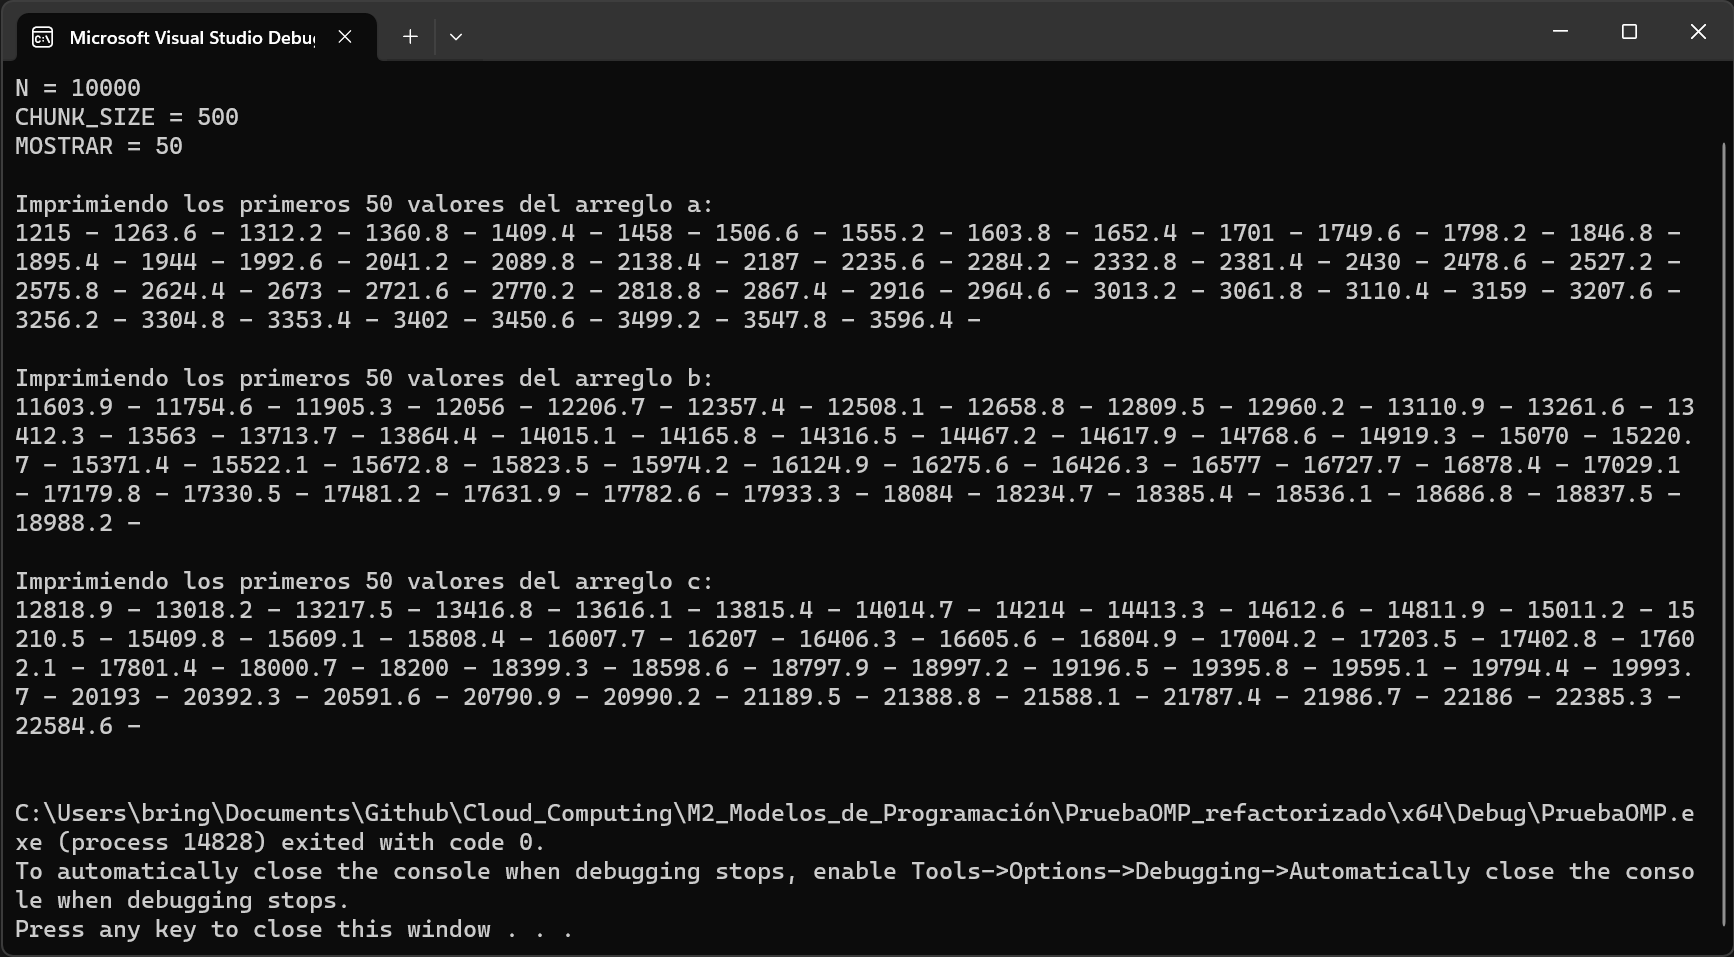
\includegraphics[width=1\linewidth]{M2_Modelos_de_Programación/reporte/figuras/Código_refactorizado_resultados.png}
    \captionof{lstlisting}{Resultados del Código refactorizado}
    \label{fig:Código_refactorizado_resultados}
\end{figure}

Como podemos observar en ambos códigos el resultado es el mismo, con lo cual se puede corroborar que las implementaciones son adecuadas y no hay discrepancias con el código refatorizado.


\section{Reflexión sobre la programación paralela}

\end{document}
